\documentclass[11pt]{article}

% --- Packages ---
\usepackage[utf8]{inputenc}
\usepackage[T1]{fontenc}
\usepackage{amsmath, amssymb, amsfonts}
\usepackage{geometry}
\usepackage{amssymb}
\usepackage{graphicx}
\usepackage{enumitem}
\usepackage{fancyhdr}
\usepackage{color}
\usepackage{hyperref}
\usepackage[most]{tcolorbox}
\usepackage{titlesec}
\usepackage{cancel} % For canceling terms
\usepackage{tikz}   % Diagrams and graphs
\usepackage{mathtools}
\usepackage{parskip}

% --- Page Setup ---
\geometry{margin=1in}
\pagestyle{fancy}
\fancyhf{}
\rhead{Algebra}
\lhead{Michael Leibbrandt}
\rfoot{\thepage}

% --- Section Styling ---
\titleformat{\section}{\large\bfseries}{\thesection}{1em}{}
\titleformat{\subsection}{\normalsize\bfseries}{\thesubsection}{1em}{}

% --- Title ---
\title{\Huge \textbf{Algebra}\\\large Notes and Practice}
\author{Michael Leibbrandt}
\date{\today}

% --- Document Begins ---
\begin{document}

\maketitle
\tableofcontents
\newpage

% ------------------------
\section{Introduction}

This document contains concise notes and worked examples.

% ------------------------
\section{Algebra Basics}

\subsection{Constants}

A \textbf{constant} is a fixed value that does not change. Unlike a \textbf{variable}, which can represent different numbers, a \textbf{constant} always has the same value.

Examples of \textbf{constant} include:

\begin{itemize}
  \item Specific numbers like \( 2 \), \( -7 \), or \( \frac{1}{2} \)
  \item Mathematical constants like \( \pi \approx 3.1416 \) or \( e \approx 2.718 \)
\end{itemize}

In the equation:
\[
x + 3 = 7
\]
the number \( 3 \) and \( 7 \) are constants — they stay the same, while \( x \) is the variable we solve for.

\subsection{Variables}

A \textbf{variable} is a symbol, usually a letter like \( x \), \( y \), or \( z \), that represents an unknown or changeable value.

For example, in the equation:
\[
x + 3 = 7
\]
the variable \( x \) represents a number. Solving the equation means finding the value of \( x \) that makes the equation true in this case, \( x = 4 \).

\textbf{Variables} are fundamental in algebra because they allow us to generalize problems and create formulas.
\subsection{Coefficients}

A \textbf{coefficient} is the numerical factor multiplied by a variable in an algebraic expression.

For example, in the term:
\[
5x
\]
the number \( 5 \) is the coefficient of the variable \( x \). It tells us how many times \( x \) is being counted or scaled.

More examples:
\begin{itemize}
  \item In \( -3y \), the coefficient is \( -3 \)
  \item In \( \frac{1}{2}a \), the coefficient is \( \frac{1}{2} \)
  \item In \( z \), the coefficient is implicitly \( 1 \), since \( z = 1 \cdot z \)
\end{itemize}

Coefficients help determine the slope of a line in linear equations and play a major role in simplifying and solving expressions.
\section{Equations vs. Expressions}

Understanding the difference between expressions and equations is essential in algebra.
\subsection{Expressions}

An \textbf{expression} is a combination of numbers, variables, and operations (like addition or multiplication), but it does \textbf{not} contain an equals sign.

Examples:
\[
2x + 5,\quad 3a^2 - 4,\quad \frac{1}{2}y
\]

Expressions represent a value, but not a complete statement to solve. You can simplify or evaluate expressions, but you cannot "solve" them unless they're part of an equation.

\subsection{Equations}

An \textbf{equation} is a mathematical statement that two expressions are equal. It always contains an equals sign (\( = \)) and usually involves finding the value of a variable that makes the equation true.

Examples:
\[
2x + 5 = 11, \quad a^2 = 16, \quad \frac{1}{2}y = 3
\]

Solving an \textbf{equation} means determining the value(s) of the variable(s) that make both sides equal.

\subsection*{Summary Table}

\begin{center}
\begin{tabular}{|c|c|}
\hline
\textbf{Expression} & \textbf{Equation} \\
\hline
No equals sign & Has an equals sign \\
Represents a value & Represents a relationship \\
Can be simplified or evaluated & Can be solved \\
Example: \( 3x + 2 \) & Example: \( 3x + 2 = 11 \) \\
\hline
\end{tabular}
\end{center}

\section{The Associative Property}

The \textbf{associative property} refers to the grouping of terms using parentheses in addition or multiplication. It tells us that the way numbers are grouped does not change the result — only the order of operations inside parentheses changes, not the outcome.

\subsection{Associative Property of Addition}

The associative property of addition states:

\[
(a + b) + c = a + (b + c)
\]

You can add numbers in any grouping, and the sum will stay the same.

\textbf{Example:}
\[
(2 + 3) + 4 = 5 + 4 = 9
\]
\[
2 + (3 + 4) = 2 + 7 = 9
\]

So, \( (2 + 3) + 4 = 2 + (3 + 4) \).

\subsection{Associative Property of Multiplication}

The associative property of multiplication states:

\[
(a \times b) \times c = a \times (b \times c)
\]

You can multiply in any grouping, and the product remains unchanged.

\textbf{Example:}
\[
(2 \times 3) \times 4 = 6 \times 4 = 24
\]
\[
2 \times (3 \times 4) = 2 \times 12 = 24
\]

So, \( (2 \times 3) \times 4 = 2 \times (3 \times 4) \).

\section{The Commutative Property}

The \textbf{commutative property} describes how the order of numbers does not affect the result when adding or multiplying. It applies only to \textbf{addition and multiplication} — not subtraction or division.

\subsection{Commutative Property of Addition}

The commutative property of addition states:

\[
a + b = b + a
\]

You can change the order of the numbers being added without changing the sum.

\textbf{Example:}
\[
4 + 7 = 11 \quad \text{and} \quad 7 + 4 = 11
\]

So, \( 4 + 7 = 7 + 4 \)

\subsection{Commutative Property of Multiplication}

The commutative property of multiplication states:

\[
a \times b = b \times a
\]

You can change the order of the numbers being multiplied without changing the product.

\textbf{Example:}
\[
6 \times 5 = 30 \quad \text{and} \quad 5 \times 6 = 30
\]

So, \( 6 \times 5 = 5 \times 6 \)
\section{Like Terms}

\textbf{Like terms} are terms that have the same variable(s) raised to the same power(s). Only the numerical coefficients can be different. Like terms can be combined using addition or subtraction.

\subsection{Addition and Subtraction of Like Terms}

To combine like terms, simply add or subtract their coefficients.

\textbf{Example 1:}
\[
3x + 5x = (3 + 5)x = 8x
\]

\textbf{Example 2:}
\[
7a^2 - 2a^2 = 5a^2
\]

\textbf{Note:} You \textit{cannot} combine terms that are not like terms.

\[
4x + 2x^2 \neq 6x^2
\quad \text{(not like terms)}
\]

\subsection{Multiplication and Division of Like Terms}

When multiplying or dividing like terms, you combine coefficients and apply exponent rules to the variables.

\textbf{Multiplication Example:}
\[
(3x)(2x) = 6x^2
\]

\[
(4a^2)(-2a^3) = -8a^5
\]

\textbf{Division Example:}
\[
\frac{10x^3}{2x} = 5x^2
\]

\[
\frac{-6y^4}{3y^2} = -2y^2
\]

\subsection*{Key Idea}

\begin{itemize}
  \item \textbf{Addition/Subtraction:} Combine only like terms (same variables and exponents)
  \item \textbf{Multiplication/Division:} Use exponent rules, even for unlike terms
\end{itemize}
\section{The Distributive Property}

The \textbf{distributive property} connects multiplication and addition or subtraction. It allows you to multiply a number or variable by each term inside parentheses.

\[
a(b + c) = ab + ac
\quad \text{and} \quad
a(b - c) = ab - ac
\]

This property is used frequently in algebra to expand expressions and solve equations.

\subsection*{Examples}

\textbf{Example 1 (with numbers):}
\[
3(4 + 5) = 3 \cdot 9 = 27
\]
\[
3 \cdot 4 + 3 \cdot 5 = 12 + 15 = 27
\]

\textbf{Example 2 (with variables):}
\[
x(2 + y) = 2x + xy
\]

\textbf{Example 3 (with subtraction):}
\[
5(a - 3) = 5a - 15
\]

\subsection*{Why It Matters}

The distributive property helps you:
\begin{itemize}
  \item Expand expressions like \( 2(x + 3) \)
  \item Simplify algebraic expressions
  \item Solve equations more efficiently
  \item Factor expressions in reverse
\end{itemize}
\subsection*{More on the Distributive Property}

The distributive property is also essential when working with variables, negative numbers, and factoring expressions.

\subsubsection*{Example with Variables and Negatives}

\[
-2(x - 4) = -2 \cdot x + (-2) \cdot (-4) = -2x + 8
\]

Notice:
\begin{itemize}
  \item The negative sign distributes to both terms
  \item Be careful with signs: \( -2 \cdot -4 = +8 \)
\end{itemize}

\subsubsection*{Common Mistake to Avoid}

Incorrect:
\[
3(x + 2) = 3x + 2 \quad \text{(Only distributed to } x \text{)}
\]

Correct:
\[
3(x + 2) = 3x + 6 \quad
\]

Always distribute to \textit{every} term inside the parentheses.

\subsubsection*{Using the Distributive Property to Factor}

The distributive property also works \textit{in reverse}, which is how we factor expressions.

\[
6x + 12 = 6(x + 2)
\]

Here, we pulled out the common factor of 6 — essentially undoing the distribution.

Factoring is the process of writing an expression as a product using the distributive property in reverse.

\textbf{Tip:} Look for a greatest common factor (GCF) before factoring!
\section{Polynomials}

A \textbf{polynomial} is an expression made up of variables, constants, and exponents, combined using addition, subtraction, and multiplication — but no variables in the denominator or under radicals.

\subsection*{Examples of Polynomials}

\[
3x^2 + 2x - 5, \quad x^3 - 4x + 7, \quad 2a^2b + 3ab^2
\]

---

\subsection{Addition and Subtraction of Polynomials}

To add or subtract polynomials:
\begin{itemize}
  \item Combine like terms (same variables raised to the same powers)
  \item Add/subtract the coefficients of like terms
\end{itemize}

\textbf{Example 1 — Addition:}
\[
(2x^2 + 3x + 1) + (x^2 + 4x - 5)
\]
\[
= (2x^2 + x^2) + (3x + 4x) + (1 - 5) = 3x^2 + 7x - 4
\]

\textbf{Example 2 — Subtraction:}
\[
(5x^2 - 2x + 6) - (3x^2 + x - 4)
\]
\[
= (5x^2 - 3x^2) + (-2x - x) + (6 + 4) = 2x^2 - 3x + 10
\]

---

\subsection{Multiplication of Polynomials}

To multiply polynomials:
\begin{itemize}
  \item Use the distributive property (FOIL for binomials)
  \item Multiply each term in the first polynomial by each term in the second
  \item Combine like terms
\end{itemize}

\textbf{Example:}
\[
(x + 2)(x + 5)
= x(x + 5) + 2(x + 5)
= x^2 + 5x + 2x + 10
= x^2 + 7x + 10
\]

\textbf{Another Example:}
\[
(2x - 3)(x^2 + x - 4)
= 2x(x^2 + x - 4) - 3(x^2 + x - 4)
\]
\[
= 2x^3 + 2x^2 - 8x - 3x^2 - 3x + 12
= 2x^3 - x^2 - 11x + 12
\]

---

\subsection{Division of Polynomials (Intro)}

Dividing polynomials can be done using:
\begin{itemize}
  \item Long division
  \item Synthetic division (when dividing by linear terms like \( x - a \))
\end{itemize}

\textbf{Basic Example:}
\[
\frac{6x^2 + 9x}{3x} = \frac{6x^2}{3x} + \frac{9x}{3x} = 2x + 3
\]

\textbf{Note:} More complex division techniques will be covered in a later section.
\begin{tcolorbox}[title=Polynomial Operations Summary, colback=blue!5!white, colframe=blue!75!black, sharp corners=southwest, boxrule=0.8pt]

\textbf{Polynomials} are expressions with variables and constants using only addition, subtraction, and multiplication (no variables in denominators or exponents).

\vspace{1ex}
\textbf{Addition/Subtraction:}
\begin{itemize}
  \item Combine like terms (same variable and exponent)
  \item Only coefficients are added or subtracted
\end{itemize}

\textbf{Multiplication:}
\begin{itemize}
  \item Use the distributive property or FOIL
  \item Multiply each term in one polynomial by each term in the other
  \item Combine like terms
\end{itemize}

\textbf{Division:}
\begin{itemize}
  \item Simplify each term if possible
  \item For complex division, use long division or synthetic division (covered later)
\end{itemize}

\end{tcolorbox}

\subsection{Long Division}

Long division is a step-by-step method for dividing numbers or algebraic expressions.

\begin{itemize}
  \item \textbf{Dividend:} the number or expression being divided
  \item \textbf{Divisor:} the number or expression you are dividing by
  \item \textbf{Quotient:} the result of the division (goes on top)
\end{itemize}

---

\subsubsection*{Example 1: Long Division with Whole Numbers}

Divide:
\[
125 \div 5
\]

Here:
\begin{itemize}
  \item Dividend = 125
  \item Divisor = 5
  \item Quotient = 25
\end{itemize}

\[
\begin{array}{r|l}
5\, &\,125 \\
\hline
& 25
\end{array}
\]

Steps:
\begin{enumerate}
  \item Divide 12 by 5 → 2 (since \( 5 \times 2 = 10 \))
  \item Subtract: \( 12 - 10 = 2 \), bring down the 5 → 25
  \item Divide 25 by 5 → 5 (since \( 5 \times 5 = 25 \))
  \item Final result: \( 25 \)
\end{enumerate}

---

\subsubsection*{Example 2: Polynomial Long Division}

Divide:
\[
\frac{x^2 + 3x + 2}{x + 1}
\]

Here:
\begin{itemize}
  \item Dividend = \( x^2 + 3x + 2 \)
  \item Divisor = \( x + 1 \)
  \item Quotient = the expression that results from division
\end{itemize}

\textbf{Step 1:} Divide leading terms:
\[
x^2 \div x = x
\]

\textbf{Step 2:} Multiply and subtract:
\[
(x^2 + 3x + 2) - (x)(x + 1) = x^2 + 3x + 2 - (x^2 + x) = 2x + 2
\]

\textbf{Step 3:} Divide leading terms again:
\[
2x \div x = 2
\]

\textbf{Step 4:} Multiply and subtract:
\[
(2x + 2) - 2(x + 1) = 2x + 2 - (2x + 2) = 0
\]

So the division is exact.

\textbf{Final Answer:}
\[
\frac{x^2 + 3x + 2}{x + 1} = x + 2
\]

---

\begin{tcolorbox}[title=Terminology Review, colback=blue!5!white, colframe=blue!75!black]
\begin{itemize}
  \item \textbf{Dividend:} what you're dividing \quad (e.g., \( x^2 + 3x + 2 \))
  \item \textbf{Divisor:} what you're dividing by \quad (e.g., \( x + 1 \))
  \item \textbf{Quotient:} result of the division \quad (e.g., \( x + 2 \))
\end{itemize}
\end{tcolorbox}
\subsection{Multivariable Polynomial Long Division}

Polynomial long division can also be performed with expressions that include more than one variable. The process is similar, but care must be taken to match like terms correctly and order terms consistently by degree.

---

\subsubsection*{Example: Divide \( 6x^2y + 9xy^2 \) by \( 3xy \)}

Here:
\begin{itemize}
  \item Dividend: \( 6x^2y + 9xy^2 \)
  \item Divisor: \( 3xy \)
\end{itemize}

\textbf{Step 1: Divide the first term of the dividend by the first term of the divisor}
\[
\frac{6x^2y}{3xy} = 2x
\]

\textbf{Step 2: Multiply the entire divisor by \( 2x \)}
\[
2x \cdot (3xy) = 6x^2y
\]

\textbf{Step 3: Subtract}
\[
(6x^2y + 9xy^2) - 6x^2y = 9xy^2
\]

\textbf{Step 4: Divide next term}
\[
\frac{9xy^2}{3xy} = 3y
\]

\textbf{Step 5: Multiply and subtract}
\[
3y \cdot (3xy) = 9xy^2
\]
\[
9xy^2 - 9xy^2 = 0
\]

\textbf{Final Answer:}
\[
\frac{6x^2y + 9xy^2}{3xy} = 2x + 3y
\]

---

\begin{tcolorbox}[title=Tips for Multivariable Long Division, colback=yellow!5!white, colframe=yellow!80!black]
\begin{itemize}
  \item Organize terms in descending order of one variable (typically \( x \))
  \item Divide one term at a time, matching both variable parts and coefficients
  \item Use standard subtraction to cancel each step before proceeding
\end{itemize}
\end{tcolorbox}
\section{Quadratic Polynomials}

A \textbf{quadratic polynomial} is a polynomial of degree 2, meaning the highest power of the variable is 2.

\subsection*{General Form}

\[
ax^2 + bx + c
\]
where:
\begin{itemize}
  \item \( a, b, c \) are real numbers and \( a \ne 0 \)
  \item \( a \) is the \textbf{leading coefficient}
  \item \( b \) is the \textbf{linear coefficient}
  \item \( c \) is the \textbf{constant term}
\end{itemize}

---

\subsection*{Examples}
\begin{itemize}
  \item \( x^2 + 5x + 6 \)
  \item \( 3x^2 - 2x + 1 \)
  \item \( -x^2 + 4 \)
\end{itemize}

---

\subsection*{Graphing Quadratics}

Quadratic functions graph as a \textbf{parabola}. The shape of the parabola depends on the sign of \( a \):
\begin{itemize}
  \item If \( a > 0 \): the parabola opens \textbf{upward} (like a smile)
  \item If \( a < 0 \): the parabola opens \textbf{downward} (like a frown)
\end{itemize}

The highest or lowest point on the parabola is called the \textbf{vertex}.

---

\subsection*{Solving Quadratic Equations}

Quadratics can be solved using several methods:
\begin{itemize}
  \item \textbf{Factoring}
  \item \textbf{Completing the square}
  \item \textbf{Quadratic formula:}
  \[
  x = \frac{-b \pm \sqrt{b^2 - 4ac}}{2a}
  \]
\end{itemize}

---

\begin{tcolorbox}[title=Quick Facts About Quadratics, colback=yellow!5!white, colframe=yellow!80!black]
\begin{itemize}
  \item Degree = 2 (because of \( x^2 \))
  \item Graph = parabola
  \item May have 0, 1, or 2 real roots depending on the discriminant \( b^2 - 4ac \)
  \item Coefficients tell you the shape and position of the graph
\end{itemize}
\end{tcolorbox}
\subsection{Factoring a Quadratic Polynomial}

Factoring is one of the most common ways to solve a quadratic equation when it can be written as a product of two binomials.

---

\subsubsection*{Example: Factor \( x^2 + 5x + 6 \)}

\textbf{Step 1:} Look for two numbers that multiply to \( 6 \) (the constant term) and add to \( 5 \) (the linear coefficient).

\[
\text{Factors of 6: } (1,6),\ (2,3)
\]
\[
2 + 3 = 5 \quad \Rightarrow \quad \text{Use } 2 \text{ and } 3
\]

\textbf{Step 2:} Write the factored form:
\[
x^2 + 5x + 6 = (x + 2)(x + 3)
\]

\textbf{Step 3:} Check by expanding:
\[
(x + 2)(x + 3) = x^2 + 3x + 2x + 6 = x^2 + 5x + 6
\]

\checkmark Confirmed!

---

\begin{tcolorbox}[title=Factoring Tips, colback=green!5!white, colframe=green!70!black]
\begin{itemize}
  \item Always look for a greatest common factor (GCF) first
  \item Use a factoring method like:
  \begin{itemize}
    \item Simple guess-and-check
    \item Box or area method
    \item AC method (for trinomials where \( a \ne 1 \))
  \end{itemize}
  \item Always double-check by expanding!
\end{itemize}
\end{tcolorbox}
\subsection{Difference of Squares}

The \textbf{difference of squares} is a special factoring pattern that applies when a binomial consists of two perfect squares being subtracted.

\[
a^2 - b^2 = (a - b)(a + b)
\]

This works because when expanded:
\[
(a - b)(a + b) = a^2 + ab - ab - b^2 = a^2 - b^2
\]

---

\subsubsection*{Examples}

\begin{itemize}
  \item \( x^2 - 9 = (x - 3)(x + 3) \)
  \item \( 4x^2 - 25 = (2x - 5)(2x + 5) \)
  \item \( 49y^2 - 1 = (7y - 1)(7y + 1) \)
  \item \(x^4 - 16 = (x^2)^2 - 4^2 = (x^2 - 4)(x^2 + 4) = (x - 2)(x + 2)(x^2 + 4) \)


\end{itemize}

---

\textbf{Important Notes:}
\begin{itemize}
  \item Works only with \textbf{subtraction}, not addition
  \item Both terms must be perfect squares
  \item Often used to simplify expressions or solve equations
\end{itemize}

---

\begin{tcolorbox}[title=Difference of Squares Summary, colback=red!5!white, colframe=red!75!black]
\[
a^2 - b^2 = (a - b)(a + b)
\]

\textbf{Examples:}
\begin{itemize}
  \item \( x^2 - 16 = (x - 4)(x + 4) \)
  \item \( 9a^2 - 1 = (3a - 1)(3a + 1) \)
\end{itemize}
\end{tcolorbox}
\subsection{Completing the Square}

To solve a quadratic equation of the form:
\[
ax^2 + bx + c = 0
\]
we can complete the square — a method that rewrites the expression as a perfect square trinomial.

---
\begin{tcolorbox}[title=What is a Trinomial?, colback=green!5!white, colframe=green!70!black]
A \textbf{trinomial} is a polynomial with three terms.

In quadratic form:
\[
ax^2 + bx + c
\]
is a trinomial.

When completing the square, we turn:
\[
x^2 + bx \quad \text{(2 terms)}
\]
into:
\[
x^2 + bx + \left( \frac{b}{2} \right)^2 \quad \text{(3 terms — a perfect square trinomial)}
\]
\end{tcolorbox}

\subsubsection*{Steps to Complete the Square (when \( a = 1 \))}

\begin{enumerate}
  \item Move the constant to the other side:
    \[
    x^2 + bx = -c
    \]
  \item Take half of the coefficient of \( x \), square it, and add to both sides:
    \[
    \left( \frac{b}{2} \right)^2
    \]
  \item Now the left-hand side is a perfect square:
    \[
    \left( x + \frac{b}{2} \right)^2
    \]
  \item Solve by taking the square root of both sides
  \item Solve for \( x \)
\end{enumerate}

---

\subsubsection*{Example: Solve \( x^2 + 6x + 4 = 0 \)}

\begin{align*}
x^2 + 6x + 4 &= 0 \\
x^2 + 6x &= -4 \\
\left( \frac{6}{2} \right)^2 &= 9 \\
x^2 + 6x + 9 &= -4 + 9 \\
(x + 3)^2 &= 5 \\
x + 3 &= \pm \sqrt{5} \\
x &= -3 \pm \sqrt{5}
\end{align*}

So the solution is:
\[
x = -3 \pm \sqrt{5}
\]

---

\begin{tcolorbox}[title=Tip for Completing the Square, colback=yellow!5!white, colframe=yellow!80!black]
\textbf{When \( a \ne 1 \)}, divide the whole equation by \( a \) first.
Completing the square is also how we derive the quadratic formula!
\end{tcolorbox}

\subsubsection*{Nature of Solutions: Real vs Complex}

After completing the square (when \( a = 1 \)), we get:
\[
x^2 + bx + c = 0 \quad \Rightarrow \quad \left(x + \frac{b}{2}\right)^2 = \left( \frac{b}{2} \right)^2 - c
\]

The number and type of solutions depend on the value of:
\[
\left( \frac{b}{2} \right)^2 - c
\]

\begin{itemize}
  \item If \( \left( \frac{b}{2} \right)^2 - c > 0 \), then \( x \) has \textbf{two real} solutions
  \item If \( \left( \frac{b}{2} \right)^2 - c = 0 \), then \( x \) has \textbf{one real} solution (a repeated root)
  \item If \( \left( \frac{b}{2} \right)^2 - c < 0 \), then \( x \) has \textbf{two complex} (nonreal) solutions
\end{itemize}

---

\begin{tcolorbox}[title=Real vs Complex Solutions from Completing the Square, colback=cyan!5!white, colframe=cyan!80!black]
Given:
\[
x^2 + bx + c = 0 \Rightarrow \left(x + \frac{b}{2} \right)^2 = \left( \frac{b}{2} \right)^2 - c
\]

Then:
\begin{itemize}
  \item \( \left( \frac{b}{2} \right)^2 - c > 0 \Rightarrow \) 2 distinct real solutions
  \item \( \left( \frac{b}{2} \right)^2 - c = 0 \Rightarrow \) 1 real solution
  \item \( \left( \frac{b}{2} \right)^2 - c < 0 \Rightarrow \) 2 complex solutions
\end{itemize}
\end{tcolorbox}
\subsubsection*{Example: Completing the Square with Imaginary Solutions}

Solve the equation:
\[
x^2 + 4x + 8 = 0
\]

\textbf{Step 1: Move the constant to the other side.}
\[
x^2 + 4x = -8
\]

\textbf{Step 2: Complete the square.}
Take half of 4 and square it:
\[
\left( \frac{4}{2} \right)^2 = 4
\]

Add 4 to both sides:
\[
x^2 + 4x + 4 = -8 + 4
\]
\[
(x + 2)^2 = -4
\]

\textbf{Step 3: Take the square root of both sides.}
\[
x + 2 = \pm \sqrt{-4}
\]
\[
x + 2 = \pm 2i
\]

\textbf{Step 4: Solve for \( x \).}
\[
x = -2 \pm 2i
\]

\textbf{Final Answer:}
\[
\boxed{x = -2 \pm 2i}
\]

---

\begin{tcolorbox}[title=Imaginary Solutions, colback=red!5!white, colframe=red!80!black]
When completing the square leads to a negative number under the square root, the equation has \textbf{two complex conjugate solutions}, involving the imaginary unit \( i = \sqrt{-1} \).
\end{tcolorbox}
\subsubsection*{Complex Conjugate Solutions and the Discriminant (When \(a=1\))}

Consider the quadratic equation:
\[
x^2 + 2x + 5 = 0
\]

Completing the square:
\[
x^2 + 2x = -5
\]
Take half of 2 and square it:
\[
\left(\frac{2}{2}\right)^2 = 1
\]
Add 1 to both sides:
\[
x^2 + 2x + 1 = -5 + 1
\]
\[
(x + 1)^2 = -4
\]

Taking the square root:
\[
x + 1 = \pm \sqrt{-4} = \pm 2i
\]

Therefore,
\[
x = -1 \pm 2i
\]

\bigskip

\textbf{Complex Conjugates:}
These solutions come in pairs called complex conjugates:
\[
a + bi \quad \text{and} \quad a - bi
\]
Here, \(a = -1\) and \(b = 2\).

\bigskip

\textbf{Discriminant:}
The discriminant is:
\[
\Delta = b^2 - 4ac
\]
For the equation:
\[
a = 1, \quad b = 2, \quad c = 5
\]
\[
\Delta = 2^2 - 4 \cdot 1 \cdot 5 = 4 - 20 = -16 < 0
\]

Since \(\Delta < 0\), the solutions are complex conjugates.

\begin{tcolorbox}[title=Summary, colback=cyan!5!white, colframe=cyan!80!black]
\begin{itemize}
  \item \(\Delta > 0\): Two distinct real solutions
  \item \(\Delta = 0\): One repeated real solution
  \item \(\Delta < 0\): Two complex conjugate solutions
\end{itemize}
\end{tcolorbox}
\subsection*{The Quadratic Formula and the Discriminant}

Any quadratic equation of the form:
\[
ax^2 + bx + c = 0
\]
can be solved using the \textbf{quadratic formula}:
\[
x = \frac{-b \pm \sqrt{b^2 - 4ac}}{2a}
\]

\bigskip

\textbf{Discriminant:}
The expression under the square root, denoted by:
\[
\Delta = b^2 - 4ac
\]
is called the \textbf{discriminant}. It determines the type of solutions:

\begin{tcolorbox}[title=Discriminant Summary, colback=yellow!5!white, colframe=yellow!80!black]
\begin{itemize}
  \item If \( \Delta > 0 \): two distinct real solutions
  \item If \( \Delta = 0 \): one real solution (a repeated root)
  \item If \( \Delta < 0 \): two complex conjugate solutions
\end{itemize}
\end{tcolorbox}

\bigskip

\textbf{Example:}
Solve \( x^2 - 2x - 3 = 0 \) using the quadratic formula.

Here, \(a = 1\), \(b = -2\), and \(c = -3\).
Compute the discriminant:
\[
\Delta = (-2)^2 - 4(1)(-3) = 4 + 12 = 16
\]

Now apply the formula:
\[
x = \frac{-(-2) \pm \sqrt{16}}{2(1)} = \frac{2 \pm 4}{2}
\]

So the two solutions are:
\[
x = \frac{2 + 4}{2} = 3 \quad \text{and} \quad x = \frac{2 - 4}{2} = -1
\]

\bigskip

\textbf{Conclusion:}
The quadratic formula is a universal method for solving any quadratic equation, and the discriminant tells you what kind of solutions to expect.
\section{The Cartesian Plane}

The Cartesian Plane is a two-dimensional coordinate system defined by a horizontal number line called the \textbf{x-axis}, and a vertical number line called the \textbf{y-axis}. These axes intersect at the \textbf{origin}, denoted as \( (0, 0) \).

Each point on the plane is represented by an ordered pair \( (x, y) \), where:
\begin{itemize}
  \item \( x \) is the horizontal value (left/right),
  \item \( y \) is the vertical value (up/down).
\end{itemize}

\begin{center}
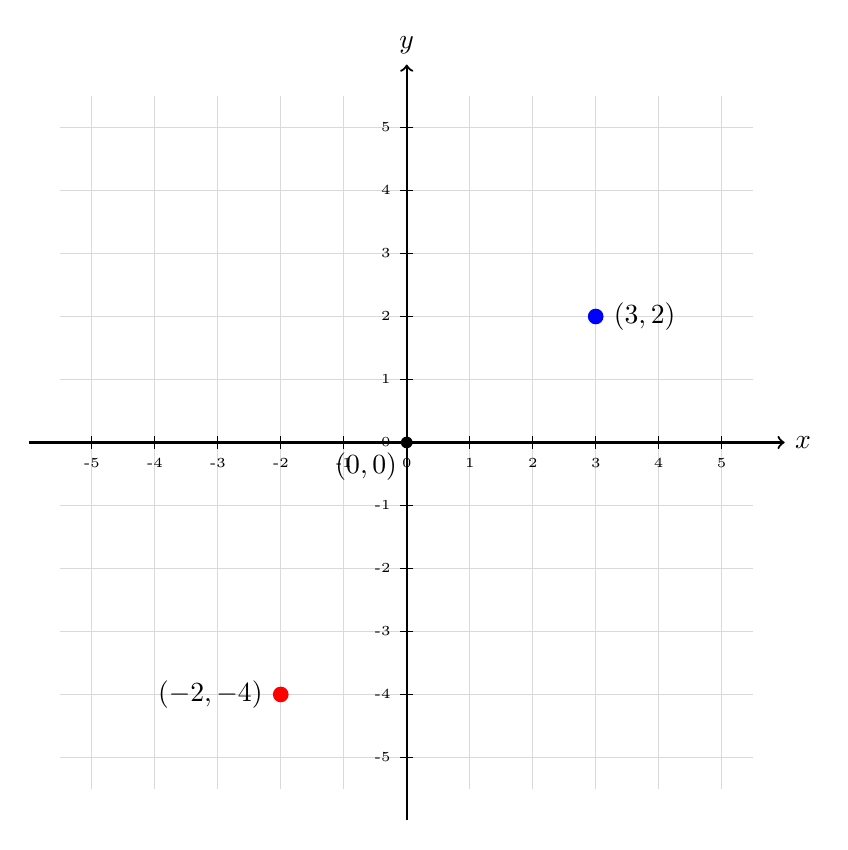
\begin{tikzpicture}[scale=0.8]
  \draw[very thin,color=gray!30] (-5.5,-5.5) grid (5.5,5.5);
  \draw[->,thick] (-6,0) -- (6,0) node[right] {\( x \)};
  \draw[->,thick] (0,-6) -- (0,6) node[above] {\( y \)};
  \node at (0,0) [circle,fill=black,inner sep=1.5pt]{};
  \node[below left] at (0,0) {\( (0, 0) \)};
  \foreach \x in {-5,-4,...,5} {
    \draw (\x,0.1) -- (\x,-0.1) node[below] {\tiny \x};
  }
  \foreach \y in {-5,-4,...,5} {
    \draw (0.1,\y) -- (-0.1,\y) node[left] {\tiny \y};
  }
  \node[circle,fill=blue,inner sep=2pt,label={right:\( (3,2) \)}] at (3,2) {};
  \node[circle,fill=red,inner sep=2pt,label={left:\( (-2,-4) \)}] at (-2,-4) {};
\end{tikzpicture}
\end{center}

\begin{tcolorbox}[colback=blue!5!white, colframe=blue!75!black, title=Summary]
\begin{itemize}
  \item The Cartesian Plane has two axes: \( x \)-axis (horizontal), \( y \)-axis (vertical).
  \item The point where they meet is the origin \( (0, 0) \).
  \item Each point is identified by an ordered pair (Called a coordinate) \( (x, y) \).
\end{itemize}
\end{tcolorbox}
\subsection{The Four Quadrants}

The Cartesian Plane is divided into four regions called \textbf{quadrants}. These are numbered in a counterclockwise direction starting from the upper-right:

\begin{itemize}
  \item \textbf{Quadrant I}: \( (+x, +y) \)
  \item \textbf{Quadrant II}: \( (-x, +y) \)
  \item \textbf{Quadrant III}: \( (-x, -y) \)
  \item \textbf{Quadrant IV}: \( (+x, -y) \)
\end{itemize}

\begin{center}
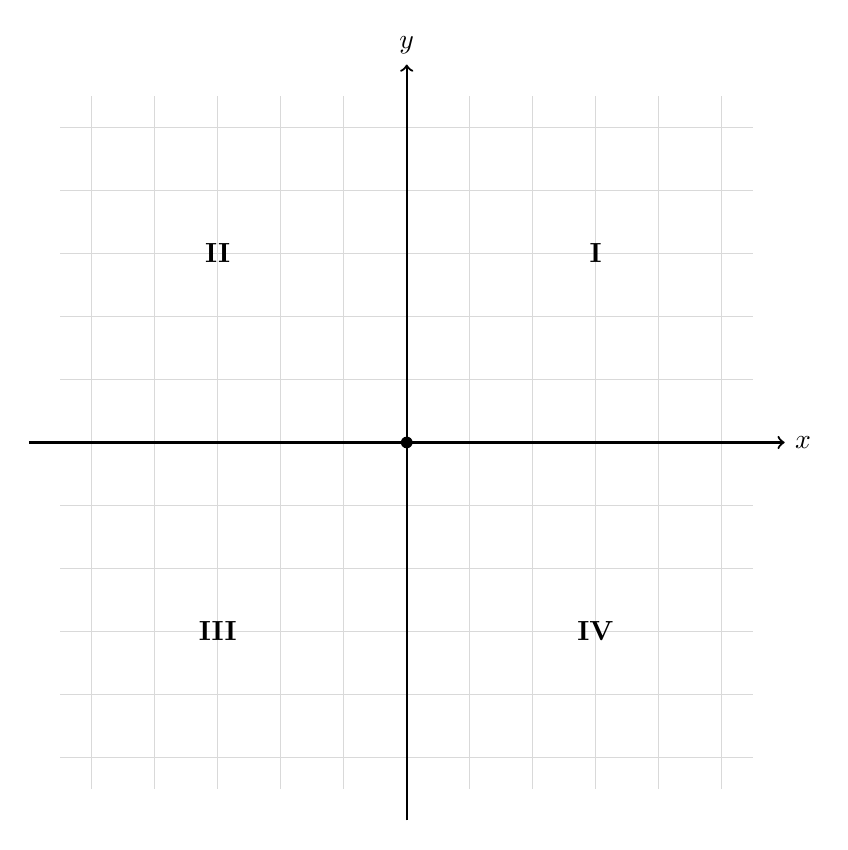
\begin{tikzpicture}[scale=0.8]
  \draw[very thin,color=gray!30] (-5.5,-5.5) grid (5.5,5.5);
  \draw[->,thick] (-6,0) -- (6,0) node[right] {\( x \)};
  \draw[->,thick] (0,-6) -- (0,6) node[above] {\( y \)};
  \node at (0,0) [circle,fill=black,inner sep=1.5pt]{};
  \node at (3,3) {\textbf{I}};
  \node at (-3,3) {\textbf{II}};
  \node at (-3,-3) {\textbf{III}};
  \node at (3,-3) {\textbf{IV}};
\end{tikzpicture}
\end{center}

\begin{tcolorbox}[colback=green!5!white, colframe=green!50!black, title=Summary of Quadrants]
\begin{itemize}
  \item Points in each quadrant have characteristic signs for \(x\) and \(y\).
  \item The quadrants are labeled I through IV, moving counterclockwise.
\end{itemize}
\end{tcolorbox}
\subsection{Slope of a Line}

The \textbf{slope} of a line is a measure of its steepness. It tells us how much the \( y \)-value changes for a given change in the \( x \)-value.

Given two points on a line, \( (x_1, y_1) \) and \( (x_2, y_2) \), the slope \( m \) is calculated using the formula:

\[
m = \frac{y_2 - y_1}{x_2 - x_1}
\]

This is also known as “rise over run”:
\begin{itemize}
  \item \textbf{Rise}: the vertical change \( (y_2 - y_1) \)
  \item \textbf{Run}: the horizontal change \( (x_2 - x_1) \)
\end{itemize}

\begin{center}
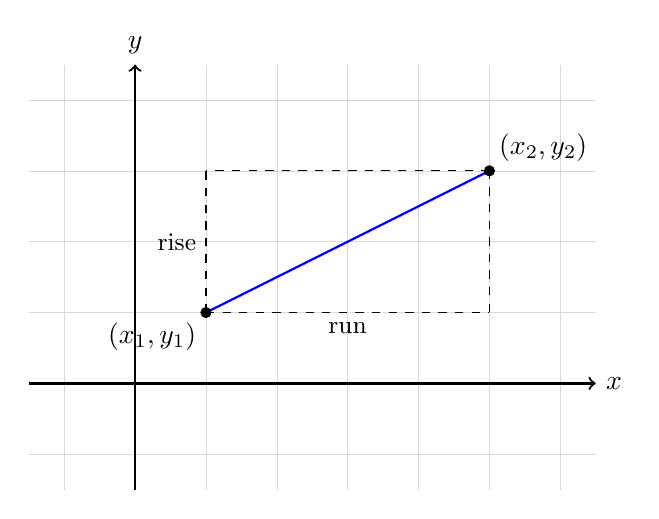
\begin{tikzpicture}[scale=0.9]
  \draw[very thin,color=gray!30] (-1.5,-1.5) grid (6.5,4.5);
  \draw[->,thick] (-1.5,0) -- (6.5,0) node[right] {\( x \)};
  \draw[->,thick] (0,-1.5) -- (0,4.5) node[above] {\( y \)};
  \coordinate (A) at (1,1);
  \coordinate (B) at (5,3);
  \draw[thick,blue] (A) -- (B);
  \filldraw[black] (A) circle (2pt) node[below left] {\( (x_1, y_1) \)};
  \filldraw[black] (B) circle (2pt) node[above right] {\( (x_2, y_2) \)};
  \draw[dashed] (A) -- ++(4,0) node[midway,below] {\small run};
  \draw[dashed] (B) -- ++(-4,0);
  \draw[dashed] (A) -- ++(0,2) node[midway,left] {\small rise};
  \draw[dashed] (B) -- ++(0,-2);
\end{tikzpicture}
\end{center}

\begin{tcolorbox}[colback=yellow!5!white, colframe=yellow!80!black, title=Summary: Slope of a Line]
\begin{itemize}
  \item Slope measures how steep a line is.
  \item Use \( m = \dfrac{y_2 - y_1}{x_2 - x_1} \) to calculate it.
  \item A positive slope rises left to right; negative slope falls.
\end{itemize}
\end{tcolorbox}

\subsection{Point-Slope Form of a Line}

If you know the slope \( m \) of a line and a point \( (x_1, y_1) \) it passes through, you can write the line's equation using the \textbf{point-slope form}:

\[
y - y_1 = m(x - x_1)
\]

\textbf{Requirements:}
\begin{itemize}
  \item A single point \( (x_1, y_1) \)
  \item The slope \( m \)
\end{itemize}

\textbf{Example:}
Given the point \( (2, 3) \) and slope \( m = 4 \), the equation becomes:

\[
y - 3 = 4(x - 2)
\]

This can be left in point-slope form or simplified to slope-intercept form.

\begin{tcolorbox}[colback=cyan!5!white, colframe=cyan!80!black, title=Point-Slope Summary]
\begin{itemize}
  \item Use when you know one point and the slope.
  \item Formula: \( y - y_1 = m(x - x_1) \)
\end{itemize}
\end{tcolorbox}

\subsection{Slope-Intercept Form of a Line}

The \textbf{slope-intercept form} expresses a linear equation as:

\[
y = mx + b
\]

Where:
\begin{itemize}
  \item \( m \) is the slope of the line.
  \item \( b \) is the \textbf{y-intercept} — the value of \( y \) when \( x = 0 \).
\end{itemize}

\textbf{Requirements:}
\begin{itemize}
  \item Slope \( m \)
  \item Y-intercept \( b \)
\end{itemize}

\textbf{Example:}
If a line has slope \( m = -2 \) and y-intercept \( b = 5 \), the equation is:

\[
y = -2x + 5
\]

This form is especially useful for graphing.

\begin{tcolorbox}[colback=orange!5!white, colframe=orange!80!black, title=Slope-Intercept Summary]
\begin{itemize}
  \item Use when slope and y-intercept are known.
  \item Formula: \( y = mx + b \)
  \item \( b \) tells you where the line crosses the \( y \)-axis.
\end{itemize}
\end{tcolorbox}
\subsection{Converting Between Forms of a Linear Equation}

Linear equations can be written in multiple forms. It’s often helpful to convert between them depending on the context (e.g., graphing, solving, or analyzing).

\subsubsection*{1. Point-Slope to Slope-Intercept}

Start with the point-slope form:
\[
y - y_1 = m(x - x_1)
\]

Distribute the slope and solve for \( y \) to convert to slope-intercept form:
\begin{align*}
y - y_1 &= m(x - x_1) \\
y &= m(x - x_1) + y_1 \quad \text{(Slope-Intercept Form: \( y = mx + b \))}
\end{align*}

\textbf{Example:}
Convert \( y - 2 = 3(x + 1) \) to slope-intercept form:
\begin{align*}
y - 2 &= 3(x + 1) \\
y - 2 &= 3x + 3 \\
y &= 3x + 5
\end{align*}

\subsubsection*{2. Two Points to Any Form}

Given two points \( (x_1, y_1) \) and \( (x_2, y_2) \):
\begin{enumerate}
  \item Find the slope \( m = \dfrac{y_2 - y_1}{x_2 - x_1} \)
  \item Use point-slope form with one point
  \item Convert to slope-intercept form if needed
\end{enumerate}

\begin{tcolorbox}[colback=purple!5!white, colframe=purple!80!black, title=Summary: Converting Forms]
\begin{itemize}
  \item Point-slope to slope-intercept: distribute and solve for \( y \)
  \item Two points → slope → point-slope → slope-intercept
  \item Use the form that best suits the problem (graphing, solving, etc.)
\end{itemize}
\end{tcolorbox}
\subsection{Undefined Slope and Vertical Lines}

A \textbf{vertical line} goes straight up and down and has an \textbf{undefined slope}. This is because its run (change in \( x \)) is zero:

\[
m = \frac{y_2 - y_1}{x_2 - x_1}
\]

If \( x_2 = x_1 \), then the denominator becomes 0, and division by zero is undefined.

\section*{Equation of a Vertical Line:}
A vertical line through \( x = a \) is written as:

\[
x = a
\]

\begin{itemize}
  \item It has an \textbf{undefined slope}.
  \item It has an \textbf{x-intercept only} — it does not cross the \( y \)-axis.
\end{itemize}

\begin{center}
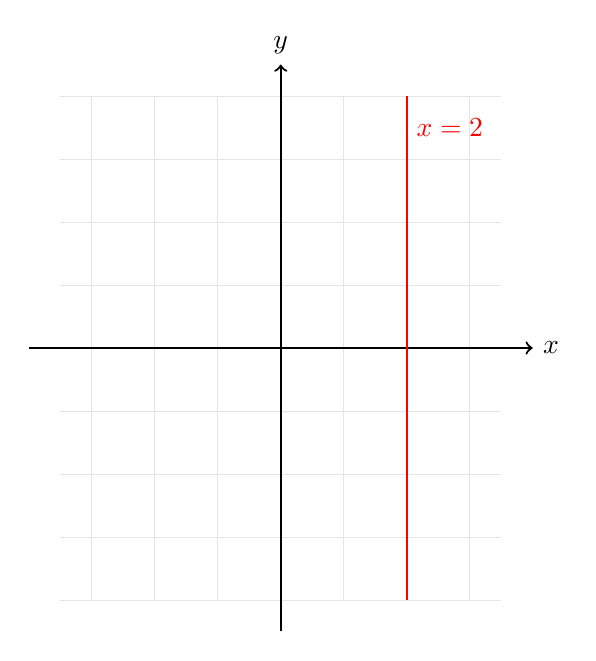
\begin{tikzpicture}[scale=0.8]
  \draw[very thin,color=gray!20] (-3.5,-4) grid (3.5,4);
  \draw[->,thick] (-4,0) -- (4,0) node[right] {\( x \)};
  \draw[->,thick] (0,-4.5) -- (0,4.5) node[above] {\( y \)};
  \draw[thick,red] (2,-4) -- (2,4);
  \node[red,right] at (2,3.5) {\( x = 2 \)};
\end{tikzpicture}
\end{center}

\begin{tcolorbox}[colback=red!5!white, colframe=red!80!black, title=Important Notes on Vertical Lines]
\begin{itemize}
  \item Vertical lines have the form \( x = a \)
  \item Their slope is undefined.
  \item They do not cross the \( y \)-axis — no \( y \)-intercept exists.
\end{itemize}
\end{tcolorbox}
\section{Graphing Linear Equations}

To graph a linear equation, such as:

\[
y = mx + b
\]

you can create a \textbf{table of values} by plugging in values for \( x \) and solving for \( y \). This gives you a set of points you can plot on the Cartesian plane.

\subsection*{Steps to Graph a Line}
\begin{enumerate}
  \item Choose three \( x \)-values (commonly: \( -1, 0, 1 \))
  \item Plug them into the equation to find corresponding \( y \)-values
  \item Plot the points \( (x, y) \) on the graph
  \item Draw a straight line through the points
\end{enumerate}

\subsection*{Example: Graph \( y = 2x + 1 \)}

\textbf{Step 1: Create a table}

\[
\begin{array}{c|c}
x & y = 2x + 1 \\
\hline
-1 & 2(-1) + 1 = -2 + 1 = -1 \\
0 & 2(0) + 1 = 0 + 1 = 1 \\
1 & 2(1) + 1 = 2 + 1 = 3 \\
\end{array}
\]

\textbf{Step 2: Plot points}

\[
(-1, -1), \quad (0, 1), \quad (1, 3)
\]

\textbf{Step 3: Draw a straight line through the points}

\begin{center}
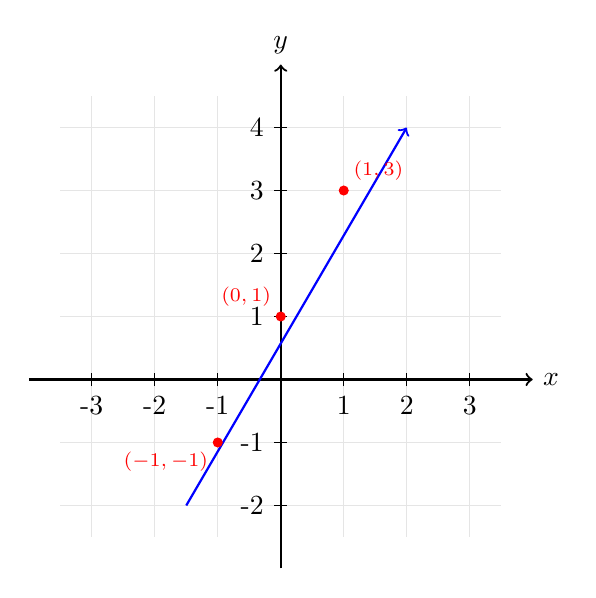
\begin{tikzpicture}[scale=0.8]
  \draw[very thin,color=gray!20] (-3.5,-2.5) grid (3.5,4.5);
  \draw[->,thick] (-4,0) -- (4,0) node[right] {\( x \)};
  \draw[->,thick] (0,-3) -- (0,5) node[above] {\( y \)};
  \foreach \x in {-3,-2,-1,1,2,3}
    \draw[shift={(\x,0)},color=black] (0pt,-3pt) -- (0pt,3pt) node[below=5pt] {\x};
  \foreach \y in {-2,-1,1,2,3,4}
    \draw[shift={(0,\y)},color=black] (-3pt,0pt) -- (3pt,0pt) node[left=5pt] {\y};

  \draw[thick,blue,->] (-1.5,-2) -- (2,4);
  \filldraw[red] (-1,-1) circle (2pt) node[below left] {\scriptsize$(-1, -1)$};
  \filldraw[red] (0,1) circle (2pt) node[above left] {\scriptsize$(0, 1)$};
  \filldraw[red] (1,3) circle (2pt) node[above right] {\scriptsize$(1, 3)$};
\end{tikzpicture}
\end{center}

\begin{tcolorbox}[colback=blue!5!white, colframe=blue!80!black, title=Graphing Summary]
\begin{itemize}
  \item Pick easy \( x \)-values: \( -1, 0, 1 \)
  \item Solve for \( y \), make a table
  \item Plot at least 3 points and draw the line
\end{itemize}
\end{tcolorbox}

\section{Functions}

A \textbf{function} is a relation where each input has exactly one output. The input is called the \textbf{independent variable} (usually \( x \)), and the output is the \textbf{dependent variable} (usually \( y \)).

Formally, a function \( f \) from a set \( A \) (domain) to a set \( B \) (codomain) assigns each element \( x \in A \) to exactly one element \( y \in B \), written as:
\[
y = f(x)
\]

\bigskip

\textbf{Key points about functions:}
\begin{itemize}
  \item For every \( x \), there is \emph{only one} corresponding \( y \).
  \item The value of \( y \) depends on the choice of \( x \).
  \item Functions can be represented by equations, tables, graphs, or mappings.
\end{itemize}

\bigskip

\textbf{Example:} Consider the function
\[
f(x) = 2x + 3.
\]
To find the output when \( x = 4 \), substitute \( 4 \) into the function:
\[
f(4) = 2(4) + 3 = 8 + 3 = 11.
\]
So, the function value at \( x = 4 \) is 11.

\bigskip

\textbf{Function notation:}
\[
f(x) = y
\]
means "the value of the function \( f \) at input \( x \) is \( y \)."


\subsection{Not a Function}

An equation is \textbf{not a function} if one input has \emph{multiple outputs}. You can test this with the \textbf{vertical line test} — if a vertical line touches the graph in more than one place, it is \emph{not} a function.

\textbf{Examples of equations that are not functions:}
\begin{itemize}
  \item \( x = 3 \) — a vertical line (undefined slope)
  \item \( x^2 + y^2 = 1 \) — a circle (one \( x \) leads to two \( y \) values)
\end{itemize}

\begin{center}
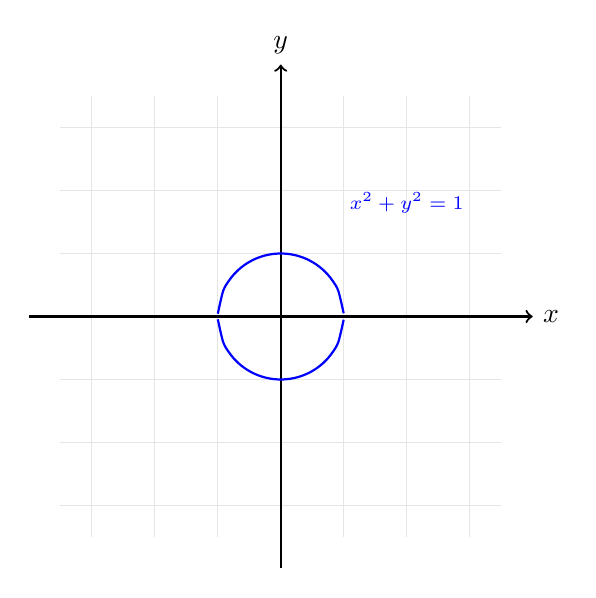
\begin{tikzpicture}[scale=0.8]
  \draw[very thin,color=gray!20] (-3.5,-3.5) grid (3.5,3.5);
  \draw[->,thick] (-4,0) -- (4,0) node[right] {\( x \)};
  \draw[->,thick] (0,-4) -- (0,4) node[above] {\( y \)};

  % Circle (Not a function)
  \draw[thick,blue,domain=-0.999:0.999,smooth,variable=\x]
  plot ({\x},{sqrt(1 - \x*\x)});
\draw[thick,blue,domain=-0.999:0.999,smooth,variable=\x]
  plot ({\x},{-sqrt(1 - \x*\x)});
  \node[blue] at (2,1.8) {\scriptsize \( x^2 + y^2 = 1 \)};
\end{tikzpicture}
\end{center}

\begin{tcolorbox}[colback=purple!5!white, colframe=purple!80!black, title=Function Summary]
\begin{itemize}
  \item A function gives exactly one output for each input.
  \item It passes the \textbf{vertical line test}.
  \item Not all equations are functions!
\end{itemize}
\end{tcolorbox}

\subsection{Domain and Range}

\textbf{Domain:} The set of all possible input values (\( x \)) for which the function is defined.

\textbf{Range:} The set of all possible output values (\( y \)) that the function can produce.

\bigskip

\textbf{How to find Domain and Range:}

\begin{itemize}
  \item \textbf{Given a function \( f(x) \):}
  Analyze the equation to determine which \( x \)-values are allowed. For example, avoid division by zero or square roots of negative numbers.

  \medskip

  \item \textbf{Given a set of points:}
  The domain is the set of all \( x \)-coordinates, and the range is the set of all \( y \)-coordinates.

  \medskip

  \item \textbf{Given a graph:}
  - The domain corresponds to all \( x \)-values covered by the graph (horizontally).
  - The range corresponds to all \( y \)-values covered by the graph (vertically).
\end{itemize}

\bigskip

\textbf{Example:}

Consider the function
\[
f(x) = \sqrt{x - 2}.
\]

\begin{itemize}
  \item \textbf{Domain:} Since the expression inside the square root must be non-negative,
  \[
  x - 2 \geq 0 \implies x \geq 2,
  \]
  so the domain is \( [2, \infty) \).

  \item \textbf{Range:} The square root outputs non-negative values, so
  \[
  y \geq 0,
  \]
  and the range is \( [0, \infty) \).
\end{itemize}

\subsection{Is It a Function? (Testing Sets of Values)}

To determine if a relation (a set of ordered pairs or an equation) is a function, use the following rule:

\begin{tcolorbox}[colback=yellow!5!white, colframe=yellow!80!black, title=Function Test]
A relation is a \textbf{function} if \emph{every input} (\( x \)-value) corresponds to \emph{exactly one output} (\( y \)-value).
\end{tcolorbox}

\textbf{Example 1 (Function — Set of Points):}
\[
\{ (1, 2), (2, 3), (3, 4) \}
\]
Each input is unique — this \textbf{is} a function.

\medskip

\textbf{Example 2 (Not a Function — Set of Points):}
\[
\{ (1, 2), (1, 3), (2, 4) \}
\]
The input \( 1 \) maps to two different outputs (\( 2 \) and \( 3 \)) — this is \textbf{not} a function.

\bigskip

\textbf{Example 3 (Algebraic Test):}

Consider the equation:
\[
x^2 + y^2 = 1
\]

Solve for \( y \):
\[
y^2 = 1 - x^2 \Rightarrow y = \pm \sqrt{1 - x^2}
\]

This gives two \( y \)-values for a single \( x \)-value.
\textbf{Conclusion:} This is \textbf{not} a function.

\bigskip

\textbf{Steps to check:}
\begin{enumerate}
  \item List all \( x \)-values or solve for \( y \).
  \item If any \( x \)-value gives more than one \( y \), it's \textbf{not} a function.
\end{enumerate}


\end{document}
